\documentclass[12pt,letterpaper]{article}
\usepackage{graphicx,textcomp}
\usepackage{natbib}
\usepackage{setspace}
\usepackage{fullpage}
\usepackage{color}
\usepackage[reqno]{amsmath}
\usepackage{amsthm}
\usepackage{fancyvrb}
\usepackage{amssymb,enumerate}
\usepackage[all]{xy}
\usepackage{endnotes}
\usepackage{lscape}
\newtheorem{com}{Comment}
\usepackage{float}
\usepackage{hyperref}
\newtheorem{lem} {Lemma}
\newtheorem{prop}{Proposition}
\newtheorem{thm}{Theorem}
\newtheorem{defn}{Definition}
\newtheorem{cor}{Corollary}
\newtheorem{obs}{Observation}
\usepackage[compact]{titlesec}
\usepackage{dcolumn}
\usepackage{tikz}
\usetikzlibrary{arrows}
\usepackage{multirow}
\usepackage{xcolor}
\usepackage{fancyvrb}
\newcolumntype{.}{D{.}{.}{-1}}
\newcolumntype{d}[1]{D{.}{.}{#1}}
\definecolor{light-gray}{gray}{0.65}
\usepackage{url}
\usepackage{listings}
\usepackage{color}
\usepackage{etoolbox}
\makeatletter
\preto{\@verbatim}{\topsep=0pt \partopsep=0pt }
\makeatother
\usepackage{placeins}



\definecolor{codegreen}{rgb}{0,0.6,0}
\definecolor{codegray}{rgb}{0.5,0.5,0.5}
\definecolor{codepurple}{rgb}{0.58,0,0.82}
\definecolor{backcolour}{rgb}{0.95,0.95,0.92}

\lstdefinestyle{mystyle}{
	backgroundcolor=\color{backcolour},   
	commentstyle=\color{codegreen},
	keywordstyle=\color{magenta},
	numberstyle=\tiny\color{codegray},
	stringstyle=\color{codepurple},
	basicstyle=\footnotesize,
	breakatwhitespace=false,         
	breaklines=true,                 
	captionpos=b,                    
	keepspaces=true,                 
	numbers=left,                    
	numbersep=5pt,                  
	showspaces=false,                
	showstringspaces=false,
	showtabs=false,                  
	tabsize=2
}
\lstset{style=mystyle}
\newcommand{\Sref}[1]{Section~\ref{#1}}
\newtheorem{hyp}{Hypothesis}

\title{Problem Set 2}
\date{Due: October 23, 2025}
\author{Ellen Beattie}

\begin{document}
	\maketitle
	
	\vspace{.5cm}
	\section*{Question 1: Political Science}
		\vspace{.25cm}
	The following table was created using the data from a study run in a major Latin American city.\footnote{Fried, Lagunes, and Venkataramani (2010). ``Corruption and Inequality at the Crossroad: A Multimethod Study of Bribery and Discrimination in Latin America. \textit{Latin American Research Review}. 45 (1): 76-97.} As part of the experimental treatment in the study, one employee of the research team was chosen to make illegal left turns across traffic to draw the attention of the police officers on shift. Two employee drivers were upper class, two were lower class drivers, and the identity of the driver was randomly assigned per encounter. The researchers were interested in whether officers were more or less likely to solicit a bribe from drivers depending on their class (officers use phrases like, ``We can solve this the easy way'' to draw a bribe). The table below shows the resulting data. \\


\begin{table}[h!]
	\centering
	\begin{tabular}{l | c c c }
		& Not Stopped & Bribe requested & Stopped/given warning \\
		\\[-1.8ex] 
		\hline \\[-1.8ex]
		Upper class & 14 & 6 & 7 \\
		Lower class & 7 & 7 & 1 \\
		\hline
	\end{tabular}
\end{table}
\newpage
\begin{enumerate}
	
	\item [(a)]
	Calculate the $\chi^2$ test statistic by hand/manually (even better if you can do "by hand" in \texttt{R}).\\
	
	\begin{itemize}
		\item  A Chi-squared test looks to determine if two categorical variables are statistically independent from each other. In this case we want to discern whether class and police response from traffic violation are statistically independent
		\item The null hypothesis $H_O$ is that the variables - Class and Encounter - are statistically independent. Our alternative $H_a$ is that they are not independent. 
		\item This is determined by looking at the observed and expected frequencies of the data. The expected frequency is the frequency that we would observe if the null was true and the variables were independent. 
		\item Our null therefore is that expected frequencies do not differ from observed frequencies. $H_O: f_O = f_e$ , and if there is not a statistical significant difference between them we have evidence supporting this hypothesis.
		\item  Alternatively, if we do find that our expected frequencies differ significantly from observed, $H_O: f_O \ne f_e$ , we have evidence to reject the null and accept that the variables are not statistically independent.   
	\end{itemize} 
	\vspace{1cm}
	
	First step is to load in data. After transferring the table data, add on a 'Total' row and column that sum up the total frequencies in each category respectively. \\
	\lstinputlisting[language=R, firstline=37, lastline=43]{PS02_EB.R} 
	\begin{verbatim}
		Observed frequency with Totals
		            Not_Stopped Bribe_Requested Stopped_Warned Total
		Upper Class          14               6              7    27
		Lower Class           7               7              1    15
		Total                21              13              8    42
	\end{verbatim}
	
	We also determine the expected frequencies of the data, which are the frequencies expected if the categories had no impact on the other variable. 
	\begin{equation}
		f_e = \frac{row\quad total}{grand\quad total} \times column\quad  total
	\end{equation}
	\lstinputlisting[language=R, firstline=46, lastline=51]{PS02_EB.R}
	\begin{verbatim}
		Expected Frequencies
		            Not_Stopped Bribe_Requested Stopped_Warned
		Upper Class        13.5            8.36           5.14
		Lower Class         7.5            4.64           2.86
	\end{verbatim}
	
	Now we compare the observed and expected frequency tables to calculate a Chi-square.
		\begin{equation}
		\chi^2 = \sum\frac{(f_O - f_e)^2}{f_e} 
	\end{equation}
	\lstinputlisting[language=R, firstline=53, lastline=55]{PS02_EB.R}
	\begin{verbatim}
		[1] 3.801141
	\end{verbatim}
	
	The overall test statistic of the Chi-squared is $\chi ^2 = 3.80$
	\vspace*{1cm}
	
	\item [(b)]
	Now calculate the p-value from the test statistic you just created (in \texttt{R}).\footnote{Remember frequency should be $>$ 5 for all cells, but let's calculate the p-value here anyway.}  What do you conclude if $\alpha = 0.1$?\\
	
	Calculate the p-value, i.e the probability of finding our Chi-square value under the null hypothesis given the degrees of freedom. 
	\lstinputlisting[language=R, firstline=59, lastline=61]{PS02_EB.R}
	\begin{verbatim}
	[1] 0.1494833
	\end{verbatim}
	
	 Since the p-value $p=0.150$ is greater than set confidence level - $p=0.150 > 0.1 = \alpha $ - we accept our null hypothesis that the two variables are statistically independent. This means we do not have evidence to accept the alternative hypothesis that class impacts the encounter when breaking traffic laws.  
	
	We can check these results with the  built-in Chi-square function in R and see they are the same (bar rounding) to our by-hand values. 
	\lstinputlisting[language=R, firstline=63, lastline=63]{PS02_EB.R}
	 \begin{verbatim}
	 	Pearson's Chi-squared test
	 	data:  fO and fe
	 	X-squared = 3.7912, df =
	 	2, p-value = 0.1502
	 \end{verbatim}
	 
	\vspace*{1cm}
	\item [(c)] Calculate the standardized residuals for each cell and put them in the table below. \\

	By calculating standardized residuals we can see how much each observed value differs from the expected. 
	This is the difference between the observed and expected frequency adjusted by the standard error of the difference under the null hypothesis. \\
	
	\begin{equation}
		z = \frac{f_O - f_e}{se} =
		 \frac{f_O - f_e)}{\sqrt[]{f_e(1-row prop.)(1- col prop.)}}
	\end{equation}\\
	
	\lstinputlisting[language=R, firstline=68, lastline=70]{PS02_EB.R}
	
	\begin{table}[h]
		\centering
		\begin{tabular}{l | c c c }
			& Not Stopped & Bribe requested & Stopped/given warning \\
			\\[-1.8ex] 
			\hline \\[-1.8ex]
			Upper class  & 0.32 & -1.52 & 1.65 \\
			\\
			Lower class & -0.27  &  1.93 & -1.52  \\
			                                              
		\end{tabular}
	\end{table}
	
	
	
	\newpage
	\item [(d)] How might the standardized residuals help you interpret the results?  \\
	\begin{itemize}
		\item 	The table is good way to quickly visualise where we find the biggest standardised differences between observed and expected frequency. This may help find out where the largest residuals are that contribute to the chi-square.
		\item Cells also have different numbers of counts and therefore those with more counts are likely to have larger residuals overall, but by standardizing them, each cell's adjusted residuals can more fairly be compared.
		\item Another benefit of standardised residuals is they because they are standardised they approximate to the standard normal distribution N(0,1), therefore can be used to conduct post-hoc tests on specific cells. 
		\item The absolute value of the cells can be compared with critical values i.e $N(0,1)_(1-\alpha/2) = 1.96 $ at $\alpha = 0.05$ level such that any standardized residuals greater than this level will be significant.
		\item Here we can see that none of the cells values have an absolute value equal to or greater than 1.96 indicating there is not a significant difference between expected and observed to a level $\alpha = 0.05$. This lines up with our overall Chi-squared result that the variables are statistically independent. 
		\item However, if we were to find that the variable were not independent with significant differences between observed and expected frequencies, this table of standardized residuals would allow us to see and analyse precisely which cells differed and by how much.   
	\end{itemize}
 
	
	
\end{enumerate}
\newpage

\section*{Question 2: Economics}
Chattopadhyay and Duflo were interested in whether women promote different policies than men.\footnote{Chattopadhyay and Duflo. (2004). ``Women as Policy Makers: Evidence from a Randomized Policy Experiment in India. \textit{Econometrica}. 72 (5), 1409-1443.} Answering this question with observational data is pretty difficult due to potential confounding problems (e.g. the districts that choose female politicians are likely to systematically differ in other aspects too). Hence, they exploit a randomized policy experiment in India, where since the mid-1990s, $\frac{1}{3}$ of village council heads have been randomly reserved for women. A subset of the data from West Bengal can be found at the following link: \url{https://raw.githubusercontent.com/kosukeimai/qss/master/PREDICTION/women.csv}\\

\noindent Each observation in the data set represents a village and there are two villages associated with one GP (i.e. a level of government is called "GP"). Figure~\ref{fig:women_desc} below shows the names and descriptions of the variables in the dataset. The authors hypothesize that female politicians are more likely to support policies female voters want. Researchers found that more women complain about the quality of drinking water than men. You need to estimate the effect of the reservation policy on the number of new or repaired drinking water facilities in the villages.
\vspace{.5cm}
\begin{figure}[h!]
	\caption{\footnotesize{Names and description of variables from Chattopadhyay and Duflo (2004).}}
	\vspace{.5cm}
	\centering
	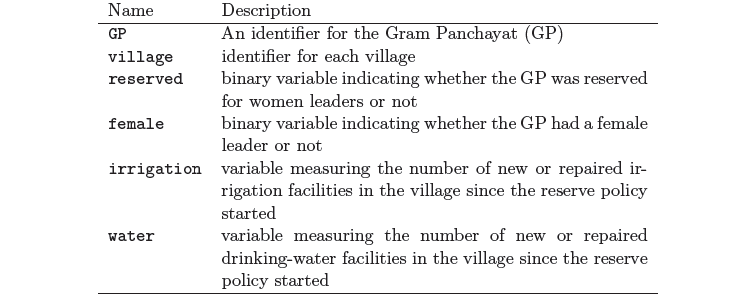
\includegraphics[width=.75\textwidth]{women_desc.png}
	\label{fig:women_desc.png}
\end{figure}
\FloatBarrier

	\lstinputlisting[language=R, firstline=80, lastline=80]{PS02_EB.R}		

\newpage
\begin{enumerate}
	\item [(a)] State a null and alternative (two-tailed) hypothesis. 
	
	\begin{itemize}
		\item Null hypothesis: Having a reservation policy has no effect on the number of new or repaired drinking-water facilities in the villages, $H_0: \beta_1 = 0$
		\item 	Alternative hypothesis: Having a reservation policy has an effect on the number of new or repaired drinking-water facilities in the villages, $ H_a: \beta_1 \ne 0$
 
	\end{itemize}
	
	\vspace{1cm}
	\item [(b)] Run a bivariate regression to test this hypothesis in \texttt{R} (include your code!).\\ 
	 
	Identify that GP is the observations $n=322$, the explanatory variable for my hypothesis is reserved ($x_1$)and the response variable is water ($Y$), such that the linear model is $Y = \alpha +\beta_1X$. 
	First step is to get familiar with the data to see sample distribution.  \\
	\lstinputlisting[language=R, firstline=88, lastline=88]{PS02_EB.R}
	\begin{verbatim}
	 summary(GP$water)
		Min. 1st Qu.  Median    Mean 3rd Qu.    Max. 
		0.00    3.00    9.00   17.84   20.00  340.00
	\end{verbatim}
	\lstinputlisting[language=R, firstline=89, lastline=89]{PS02_EB.R}
	\begin{verbatim}
		> count(GP$reserved)
			x freq
			1 0  214
			2 1  108
	\end{verbatim}
	\lstinputlisting[language=R, firstline=90, lastline=96]{PS02_EB.R}
		\begin{figure}[!htbp]\centering
		\caption{\footnotesize Distribution plots of Explanatory and Response variables}
		\label{fig:plot_1}
		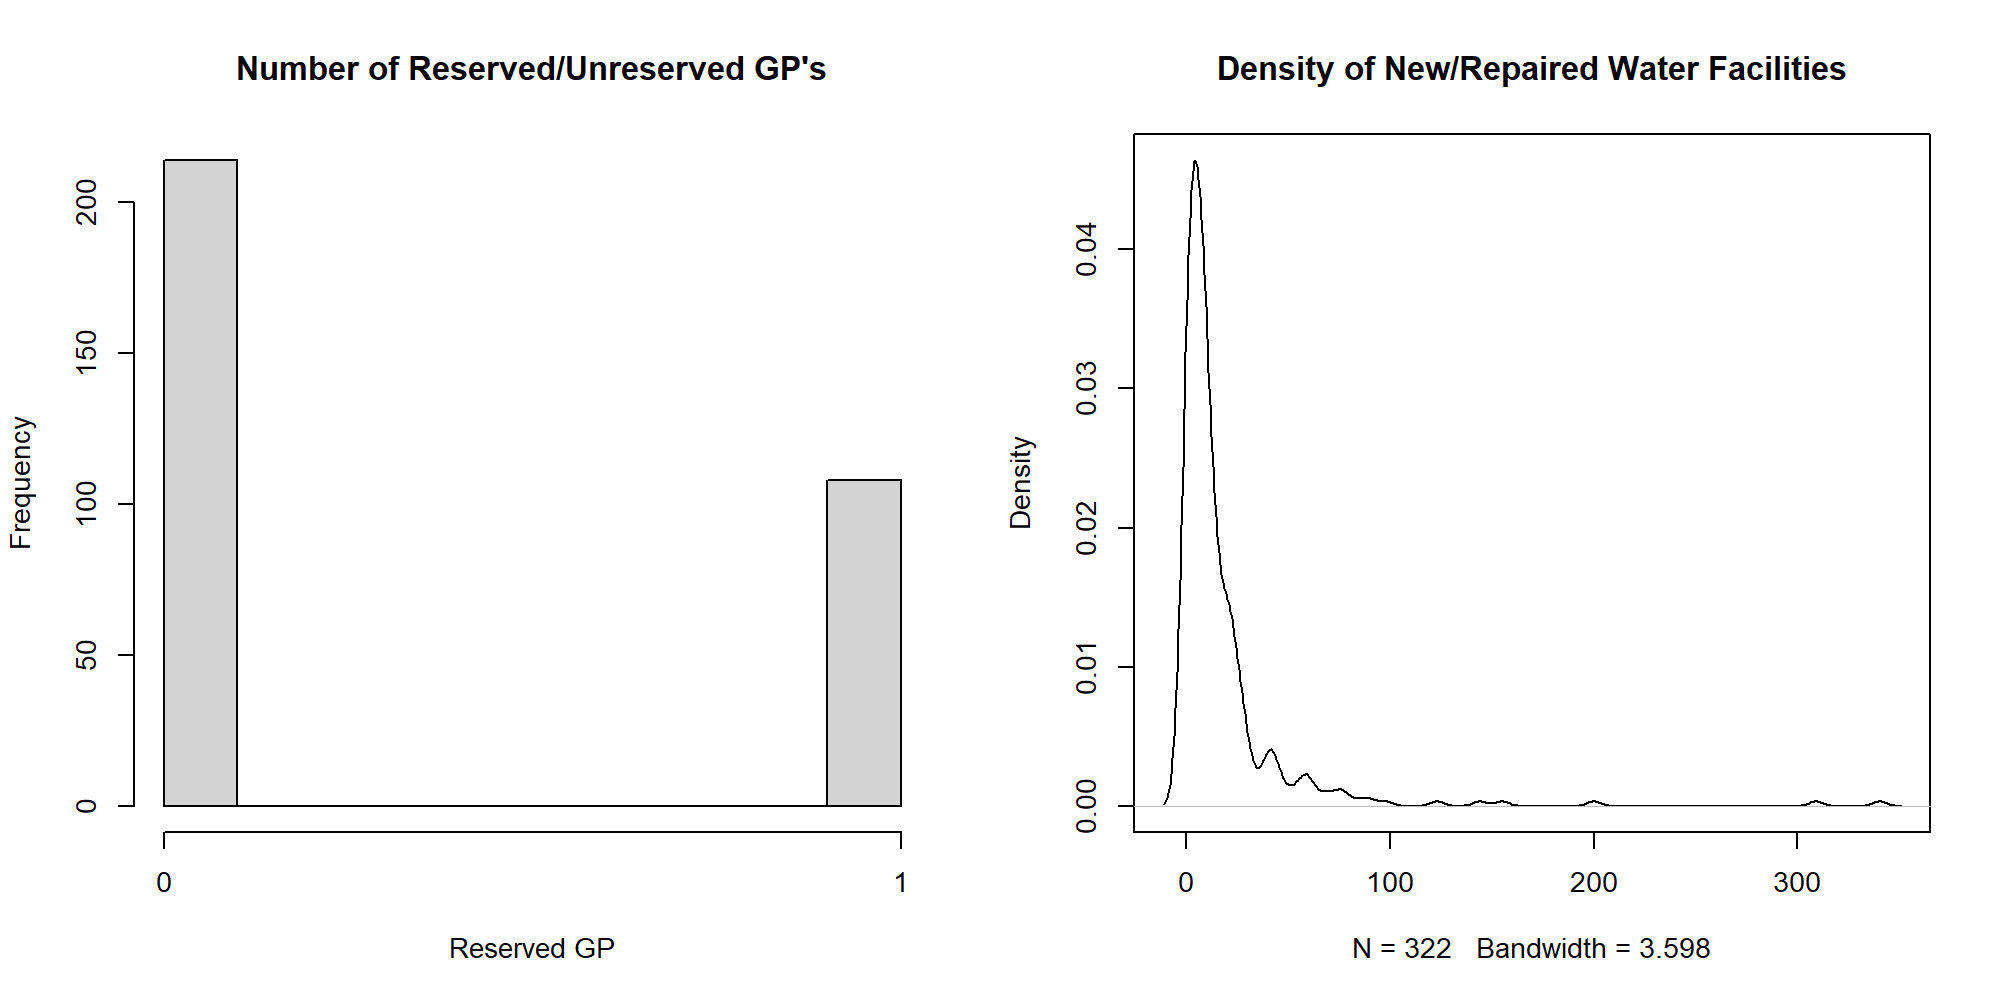
\includegraphics[width=.8\textwidth]{PS02_explore.png}
	\end{figure}
	\FloatBarrier
	From this initial investigation we can see that reserved is a binary variable, i.e  1 indicating a reserved GP and 0 indicating it is not reserved for women. We can see that there are roughly double the number of unreserved GP's to reserved.
	We can also see the distribution of Y that there is a positive skew.  The mean is $\bar{y}= 17.84$ and the median is $9$ indicating the impact of larger values increasing the mean, consistent with the seen positive skew. There does appear to be a few outliers with very high values (like the max of 340) that is important to be aware of going into the regression. \\
	
	
	\lstinputlisting[language=R, firstline=100, lastline=115]{PS02_EB.R}

	\input{PS02_reg1output.tex}
	\FloatBarrier
	\begin{figure}[!htbp]\centering
		\caption{\footnotesize Plot of Water and Reserved Policy}
		\label{fig:plot_1}
		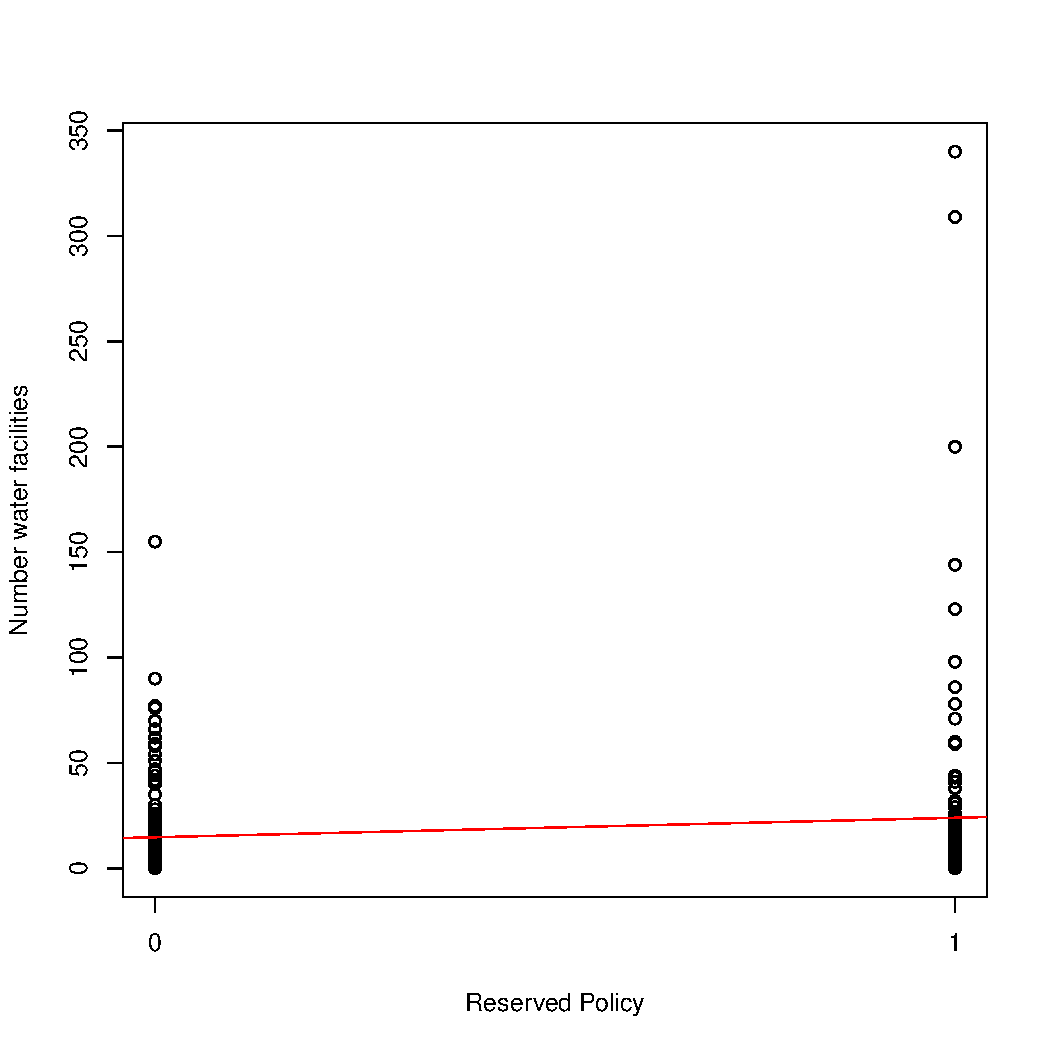
\includegraphics[width=.65\textwidth]{PS02_Reg_Plot.pdf}
	\end{figure}
	\FloatBarrier
	
	\lstinputlisting[language=R, firstline=118, lastline=118]{PS02_EB.R}
	\begin{verbatim}
		Coefficients:
													Estimate 		Std.Error 		t value 		Pr(>|t|)    
		(Intercept)   14.738      2.286   	6.446 		4.22e-10 ***
		reserved       9.252      3.948   	2.344   	0.0197 *  
		---
		Signif. codes:  0 ‘***’ 0.001 ‘**’ 0.01 ‘*’ 0.05 ‘.’ 0.1 ‘ ’ 1
		
		Residual standard error: 33.45 on 320 degrees of freedom
		Multiple R-squared:  0.01688,	Adjusted R-squared:  0.0138 
		F-statistic: 5.493 on 1 and 320 DF,  p-value: 0.0197
	\end{verbatim}
	\vspace{1cm}
	\item [(c)] Interpret the coefficient estimate for reservation policy. 
	\begin{itemize}
		\item 	The coefficient estimate is the slope of the best fit regression line from the model, i.e. how a change in one variable is associated with another, in this case looking at reservation policy on water facilities.
		\item The coefficient estimate $\hat\beta_1=9.525$ can be interpreted as having a reservation policy (a 1 unit increase for binary variable) is associated with 9.252 increase in the number of new or repaired drinking-water facilities.
		\item Our coefficient estimate is point estimate that we have used to make a best guess as to the true unknown population parameter. We need to therefore summarize just how well our estimate supports our hypothesis allowing us to make inferences about the population. 
		\item From our model we can see the standard error of the estimate $se_(\hat\beta_1) = 3.948$. This indicates the uncertainty of the estimate, i.e if we were to conduct repeated sampling how much do we expect the coefficient to differ. 
		\item We can test our estimate by using the t-distribution to compare a calculated t-score to a relevant critical value given our null ($H_0: \beta_1 = 0$); \begin{equation}
			t = \frac{\hat{\beta}_1 -0}{se_(\hat{\beta}_1)} = \frac{9.252}{3.948} = 2.344 \sim t_{n-2}
		\end{equation}
		\item  To calculate p-value we use two-tailed probability from t-distribution
			\begin{equation}
				p-value = 2 \times Pr(t_{320} > |2.344|) = 0.0197
				\end{equation}
		\item At $\alpha= .05$ we are able to reject the null hypothesis as $p <0.05$ and accept the alternative that $\beta_1$ is statistically differentiable from 0 i.e.  that having a reservation policy does impact the number of new or repaired drinking-water facilities in a village. 
		\item We can also construct a 95\% confidence interval for our found estimate
		\lstinputlisting[language=R, firstline=113, lastline=113]{PS02_EB.R}
		\begin{verbatim}
																		2.5 %   97.5 %
			(Intercept) 10.240240 19.23640
			reserved     1.485608 17.01924
		\end{verbatim}
		\item 	Thus a 95\% confidence interval of the estimate with $t_{320}$ is [1.49,17.02] which does not include zero, further confirming our rejection of the null hypothesis. We can also conclude that at the 95\% confidence level, having a reservation policy increases the number of new/repaired drinking water facilities by as few as 1.49 facilities or as many as 17.02 facilities. 
		 
	\end{itemize}

\end{enumerate}


\end{document}
